\chapter{Solution Design: Improved Kepler Visualisation Tool (IKVT)}\label{C:sd}
This section discusses the design of the deliverable visualisation, the Improved
Kepler Visualisation Tool (IKVT). It details
the key design decisions revolving around structure, aesthetics, and
functionality that were made about the visualisation. 
% Description of tool
This project aimed to improve an existing visualisation, The Kepler Visualisation
Tool which was discussed in the previous chapter. This 
visualisation displays exoplanets and some of their features but lacks effective
interactivity for users to access the detailed information contained in the
Kepler Exoplanet Database. The IKVT expands on this pre-existing
visualisation by adding key elements of interactivity missing in the existing
 visualisation as well as further enhancing the range and amount of data that
is available to users. The IKVT also incorporates a novel
gesture based interactive mechanism for controlling the visualisation using a
Microsoft
Kinect Sensor.

\section{System Design and Structure}
As this project builds upon the Kepler Visualisation
Tool, complete comprehension of
how it is designed and how it functions is important. Going ahead in extension
without this knowledge would create opportunities
for mistakes and incorrect assumptions. To solve this issue diagrams using the
Unified Modeling Language(UML) were used. In UML there are two basic categories
of diagrams: structure diagrams and
behavior diagrams. Every UML diagram belongs to one these two diagram
categories. The purpose of structure diagrams is to show the static structure of
the system being modeled i.e. class diagrams, and object diagrams. Behavioral
diagrams show the dynamic behavior between the objects in
the system, including aspects like their methods, collaborations, and activities
i.e. use case and sequence diagrams \cite{ibm}. For this project sequence
diagrams and class diagrams were used to
understand the existing system and plan out the extensions, these are discussed
next.

\begin{enumerate}
\clearpage
{\bf \item UML Sequence Diagram}
  A sequence diagram primarily shows the interactions between
objects in the sequential order that those interactions occur.
For this project it was used to understand how each of the objects in the system
worked together to create the visualisation. Without understanding which objects
were responsible for each part of the render cycle it would have been difficult
to extend the visualisation. Through the sequence diagram we can see when each
of the objects in the system are updated, and when they are rendered. 
   \begin{figure}[H]
  \centering
      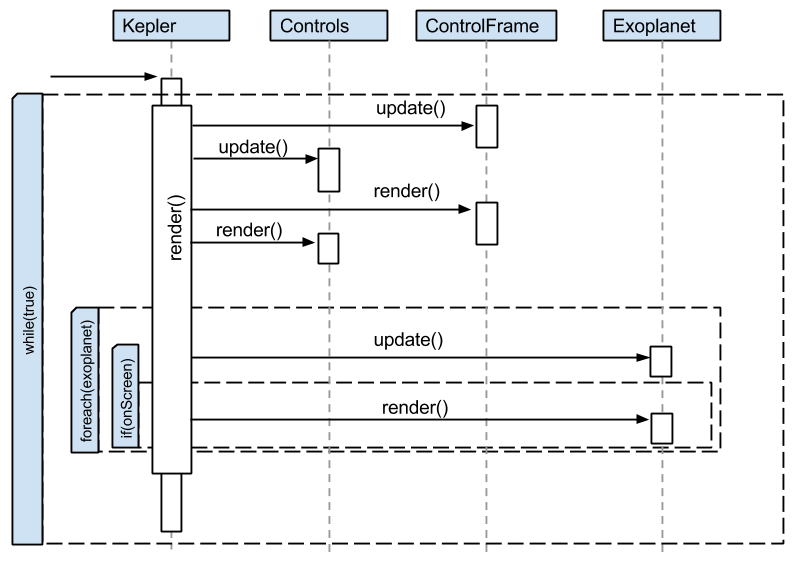
\includegraphics[width=1\textwidth]{images/sequence.png}
  \caption[Sequence Diagram of IKVT render cycle]{Sequence Diagram of IKVT
render cycle, it shows when each component of the visualisation is updated and
rendered.}  
    \label{fig:sequenceDiagram}
\end{figure}
\clearpage
 {\bf \item UML Class Diagram}
 Class diagrams describe the structure of a system by showing the systems
classes, their attributes, methods, and the relationships among objects.
 Developers can use class diagrams to design and document the systems coded (or
soon to be coded) classes. For this project class diagrams were used to
understand
the makeup of the existing Kepler Visualisation Tool and then to plan the
extensions. The diagram in Figure \ref{fig:classDiagram} shows the structure and attributes of the Kepler Visualisation Tool. This class
diagram was updated with the improvements introduced in the visualisation
to provide an overview that could be used for further planning.
 \begin{figure}[H]
  \centering
      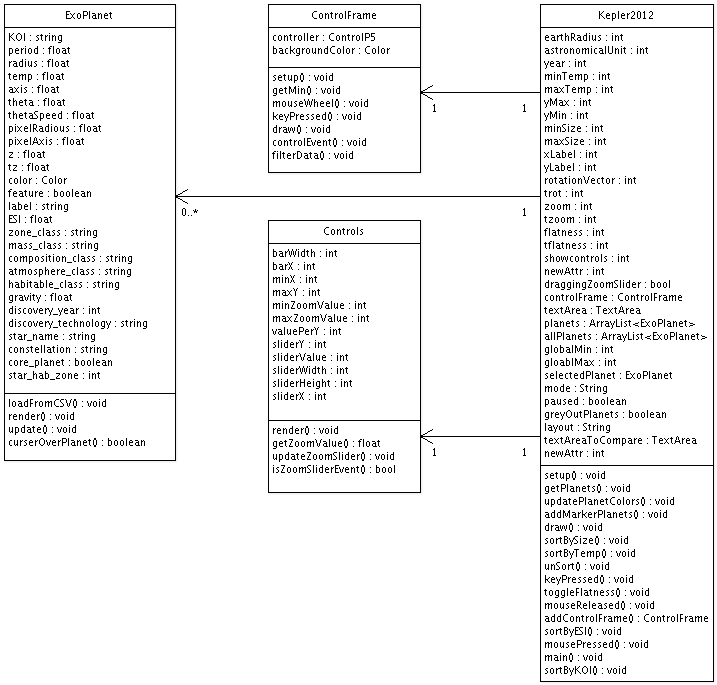
\includegraphics[width=0.8\textwidth]{images/classDiagram.png}
  \caption[Class Diagram of IKVT]{The class diagram used to understand
the structure of the existing Kepler Visualisation Tool and plan the
extensions.}  
  \label{fig:classDiagram}
\end{figure}
\end{enumerate}

By using
the sequence diagram in Figure \ref{fig:sequenceDiagram} coupled with the class
diagram in Figure \ref{fig:classDiagram} we can see where each method and field
is located and modified. This is a powerful way to understanding an
existing system and then planning extensions.

\section{Visualisation Design}
The requirements produced in Chapter \ref{Chap:ra}: Requirements Analysis
provide a
description of the functionality needed for this
visualisation. By adding additional details to these requirements we can specify
how the visualisation should look, behave, and function. This is done in the
following subsections.

\clearpage
\subsection{Functional Requirements}
\begin{enumerate}

{\bf
 \item[R1.] The visualisation needs to display planetary information to convey
knowledge to users.
}

  This requirement needs a textual display in order to convey information about
exoplanets to the user. This can be done with a Java
text area object to display each of the key
attributes of exoplanets. The following figure is an example of the text area
showing the information about each planet that would be displayed and the method
calls that would be used.

\begin{figure}[H]
  \centering
      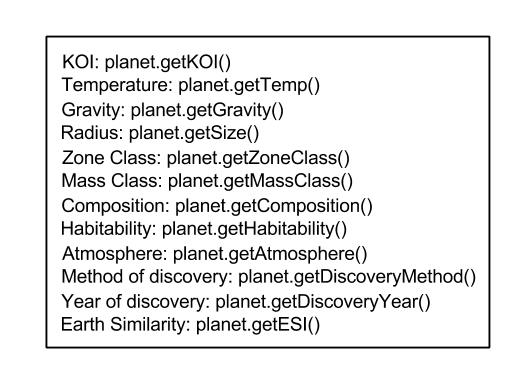
\includegraphics[width=0.8\textwidth]{images/textAreaMockup.png}
  \caption[Example of the text area]{Example of the text area that displays
information about selected exoplanets. Also included are the planned method
calls for populating the fields}
  \label{fig:text}
\end{figure}


\clearpage
{\bf
 \item[R2.] The visualisation needs to allow exoplanets to be compared against
one another.}

There are two steps to fulfilling this requirement\\ {\bf1.} Allow selection of
exoplanets \\ {\bf2.} Display additional information about exoplanets when they
are
selected.

The selection of exoplanets involves detecting when and where a user clicks, and
then 
finding whether any planets are
located in that space. This is more complex in this system as it requires
detecting if the 3D space of each planet coincides with the 2D
location of the mouse click. When a planet is successfully selected it needs to
provide feedback to the user to inform them that it has been selected and also
to
provide information about the selected exoplanet as in Figure \ref{fig:text}.

\begin{figure}[H]
  \centering
      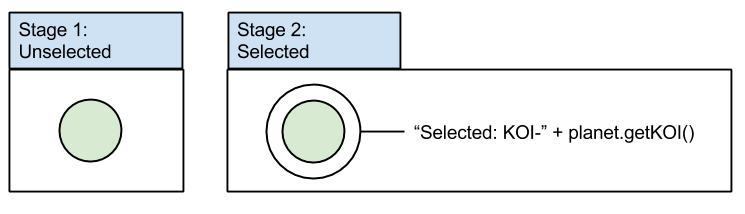
\includegraphics[width=.8\textwidth]{images/mockSelected.png}
  \caption[Example of exoplanet selection process]{Example of exoplanet
selection process. It displays the result of an exoplanet being selected, first
the planet expands, then a white circle expands out to outline it.}  
\end{figure}

In addition to this, when a planet has been selected all 
other planets in the
same solar system (sister planets) need to become highlighted. This can be done
by treating them as if they were selected and providing an additional indication
 to the user why they were highlighted as in Figure \ref{fig:sister}.  
\begin{figure}[H]
  \centering
      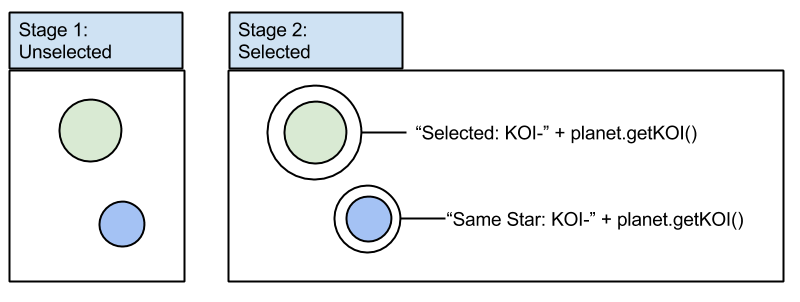
\includegraphics[width=.8\textwidth]{images/selectedSisterPlanets.png}
  \caption[Example of exoplanets in the same solar system]{Example of exoplanets
in the same solar system. It displays how the planets in the same solar system
as the selected planet become highlighted.}  
  \label{fig:sister}
\end{figure}

There needs to be an efficient way for users to make comparisons between the
detailed textual information of exoplanets. By providing an additional text
box and allowing users to select multiple planets this can be accomplished as
shown in Figure \ref{fig:comp}.

\begin{figure}[H]
  \centering
      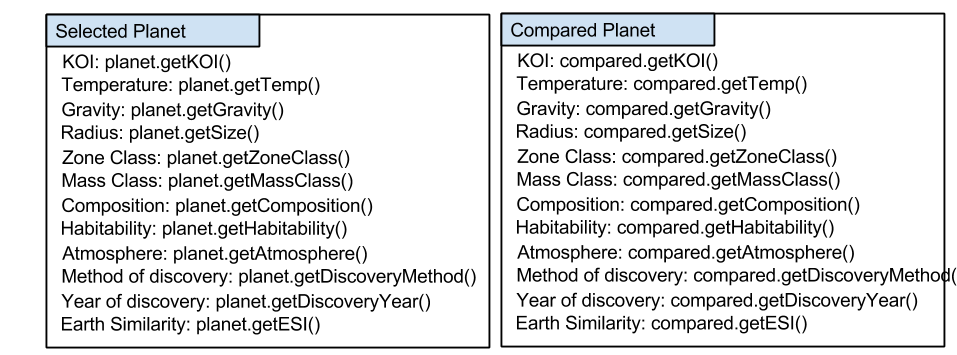
\includegraphics[width=.7\textwidth]{images/mockComparePlanets.png}
  \caption[Example of exoplanet comparison]{Example of exoplanet comparison
text areas, included are the planned method calls for populating the fields of
the second text area}
  \label{fig:comp}
\end{figure}
\clearpage

{\bf
 \item[R3.] The planets need to be able to be ordered by their similarity to
earth (ESI) and by their Kepler Object of Interest number (KOI).}

The visualisation needs to allow users to view the
exoplanets in a way that uses the Earth as a point of reference and their Earth
Similarity Index (ESI) to order them and control their position. Figure
\ref{fig:esiMock} displays an example of how this would be done.

\begin{figure}[H]
  \centering
      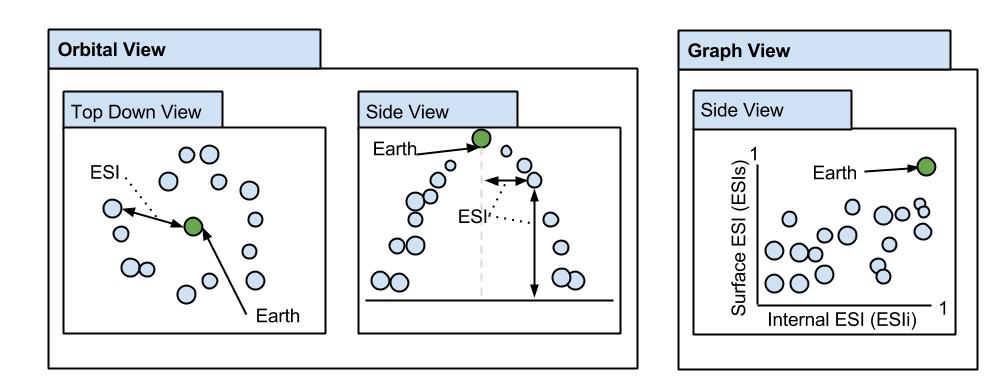
\includegraphics[width=1\textwidth]{images/mockupESI.png}
  \caption[Example of ESI views]{Example of ESI views, it shows how the ESI is
used to order the exoplanets in the orbital and graph views.}
  \label{fig:esiMock}
\end{figure}

\clearpage
{\bf
 \item[R4.] The visualisation needs to allow users to define ranges of planetary
attributes to filter which planets are displayed.}

A method of filtering the exoplanets displayed to the user is needed. A
common method of achieving this is to use a set of sliders that allow a user to
filter something by a set of values. In this system sliders would
be used to control the planets displayed by the exoplanet attributes: size,
temperature, Kepler Object of Interest number (KOI), and Earth Similarity Index
(ESI) as in Figure \ref{fig:mockSlider}.
\begin{figure}[H]
  \centering
      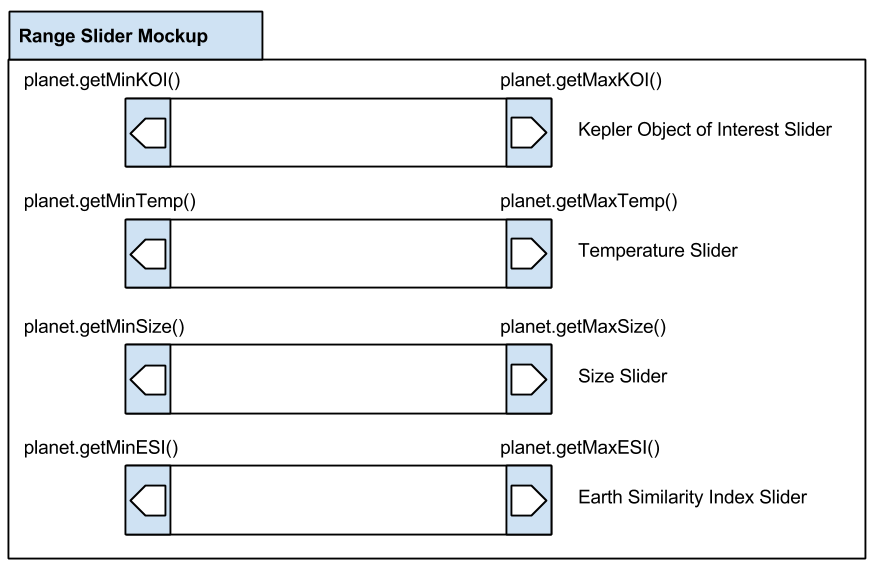
\includegraphics[width=.8\textwidth]{images/mockSlider.png}
  \caption[Example of range sliders]{Example of range sliders, it displays the
method calls used for the ranges}  
  \label{fig:mockSlider}
\end{figure}

In addition to this users should be able to sort the exoplanets to make
the most of the filtering. By allowing users to display the exoplanets sorted
vertically by the same attribute as the filters, they can see how
changing the filters affects the exoplanets displayed as exoplanets on either
side of the specified range are omitted. This would be achieved by a set of
interactive buttons as in Figure \ref{fig:mockButtons}.

\begin{figure}[H]
  \centering
      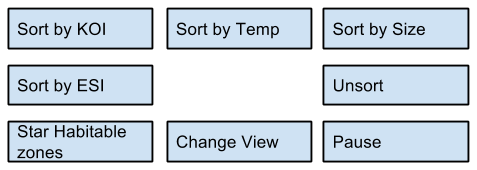
\includegraphics[width=0.5\textwidth]{images/mockButtons.png}
  \caption[Example of interactive buttons]{Example of interactive buttons
displaying each of the key interactive functions}  
  \label{fig:mockButtons}
\end{figure}

\clearpage
{\bf
 \item[R5.] Users need to be able to view the habitable zones (Goldilocks zones)
of stars in
relation to the planets orbiting them.
}

To view the Goldilocks zone each exoplanets star requires a way to display
the hot (to close to the star), cold (to far from the star), and the habitable
zone (in between hot and cold zones). This can be done by showing
the selected exoplanet in relation to its star by means of coloured circles
depicting where the exoplanet sits inside the zones, as displayed in Figure
\ref{fig:hab}. 

\begin{figure}[H]
  \centering
      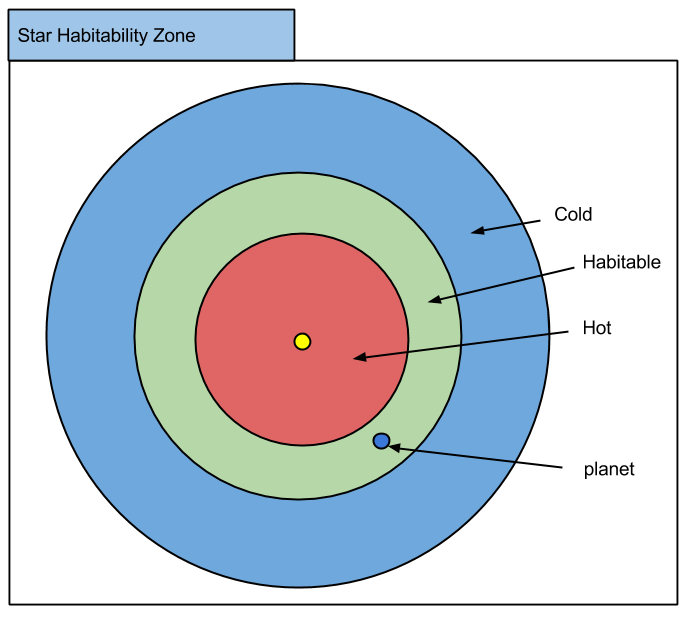
\includegraphics[width=.5\textwidth]{images/mockStarHabitability.png}
  \caption[Example of Goldilocks zones]{Example Goldilocks zones showing how the
coloured rings are used and how the planets relation to them infers their
habitability.}  
  \label{fig:hab}
\end{figure}




\end{enumerate}
\clearpage
\subsection{Nonfunctional Requirement}

\begin{enumerate}


{\bf \item[R6.] All interaction methods must be visible and intuitive.}

To make an interactive visualisation usable the controls and interactive
methods need to be clear to users. To achieve this for IKVT an interactive
control panel
is introduced. This panel contains all of the interactive elements
of the visualisation in a single central place that is spatially separated from
the main visualisation. This spacial separation is important as it reduces
cognitive load on users \cite{InformationCapacity}. It does this by allowing them to focus on the
visualisation itself
until they need to use the control panel in which case they can switch focus to
that \cite{mendel}. It also
means that users only need to look in one place for all of the interactive
elements which reduces the risk of confusion. The
control panel would contain all of the interactive elements as discussed in
the previous requirements as displayed below in Figure
\ref{fig:interactionPanelMock}.

\begin{figure}[H]
  \centering
      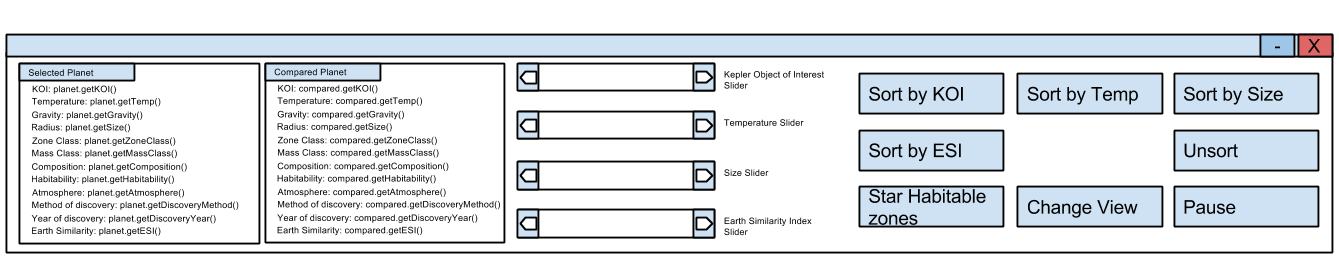
\includegraphics[width=1\textwidth]{images/allTogether.png}
  \caption[Example of the control panel]{Example of the control panel showing
the placement of each of the components talked about previously.}  
  \label{fig:interactionPanelMock}
\end{figure}

In the gesture based system intuitivity can be achieved by reusing effective and
widely recognised gestures from other visualisations. In this case these would
be push, pull, sweep left/right, raise, lower, and hover.
\clearpage
{\bf \item[R7.] The visualisation must remain uncluttered.}

The visualisation must not show so much information that it
causes information overload for users. The ability to filter and sort the
exoplanets gives a user the tools needed to
reduce the quantity of planets displayed in the visualisation and thus the
information load imposed on users \cite{lewis}. In addition to this, having the control
panel separate from the main visualisation reduces the cognitive
load on users as they don't have to use this component until they want to.
Having the interaction broken up into three sections also assists with this as it
utilises Gestalt's law of proximity \cite{withinSubject} which states that when an
individual perceives an assortment of objects close together they are seen a
group. This layout is shown in Figure \ref{fig:clutter}.

\begin{figure}[H]
  \centering
      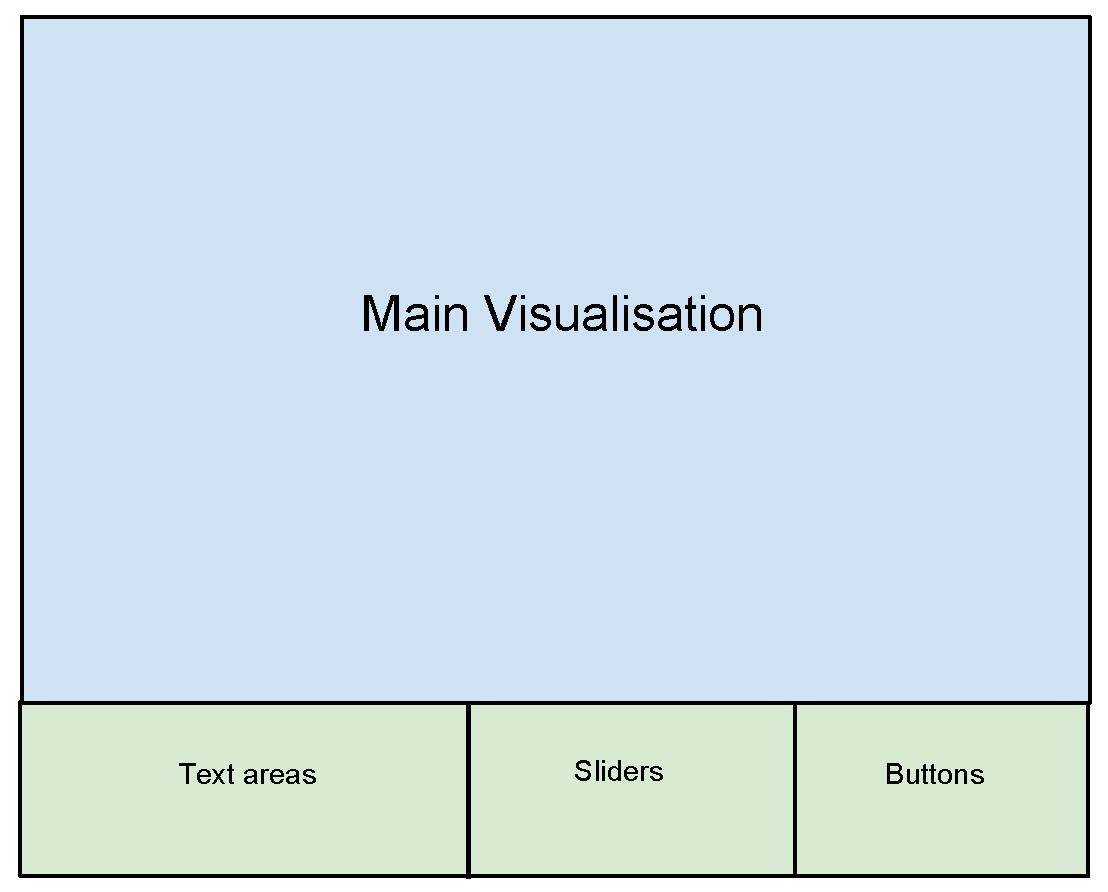
\includegraphics[width=0.8\textwidth]{images/clutter.pdf}
  \caption[Layout of visualisation]{Layout of visualisation showing how each
element is arranged to utilise grouping of similar components}
  \label{fig:clutter}
\end{figure}

\clearpage
{\bf  \item[R8.] There needs to be two modes of interaction in the system,
keyboard \& mouse vs gesture based.}

Incorporating a novel interactive method using a Microsoft Kinect sensor
gives users an alternative method of controlling the visualisation. This
requires incorporating a
means of detecting the gestures of users and linking them to an action in the
visualisation. A simple way to do this is to provide an area for the user to
gesture to on the screen that controls the movement of the camera in the
visualisation as shown in Figure \ref{fig:kinectMock}.
\begin{figure}[H]
  \centering
      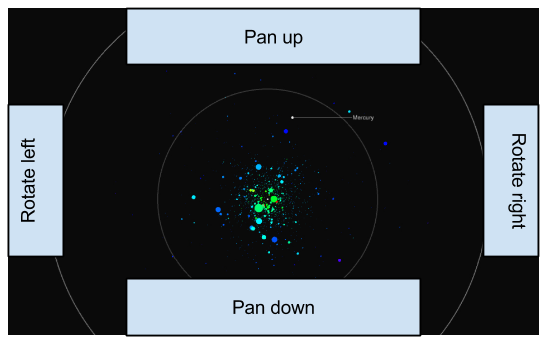
\includegraphics[width=0.7\textwidth]{images/mockKinect.png}
  \caption[Example of the Kinect system]{Example of the Kinect system showing
where the user gestures to for moving the camera in the visualisation}
  \label{fig:kinectMock}
\end{figure}

Users also need to be able to
zoom in and out of the visualisation as well as select exoplanets for further
examination. To do this users should be able to
push and pull their hand from the screen to zoom in and out, as well as
hover over a planet to make a selection. Providing feedback to users is important in keeping them informed about the
state of the visualisation, this means
incorporating new cursors to indicate the gestures that have been detected.
There are seven states that the cursor needs to be able to display to inform the user
of what action they are performing. These states are

\begin{enumerate}
\item[1.]  {\bf Default cursor, hand is at rest or hovering over a planet}
 \item[2.] {\bf Panning up, hand is raised}
 \item[3.] {\bf Panning down, hand is lowered}
 \item[4.] {\bf Rotating left, hand is to the left}
 \item[5.] {\bf Rotating right, hand is to the right}
 \item[6.] {\bf Zooming in, hand is pressed forward}
 \item[7.] {\bf Zooming out, hand is pulled backwards}
 
\end{enumerate}
Having a range of icons that clearly display these states is vital for keeping
the user informed of what they are doing. The proposed cursor icons for this are
displayed in Figure \ref{fig:cursors}
\begin{figure}[H]
  \centering
      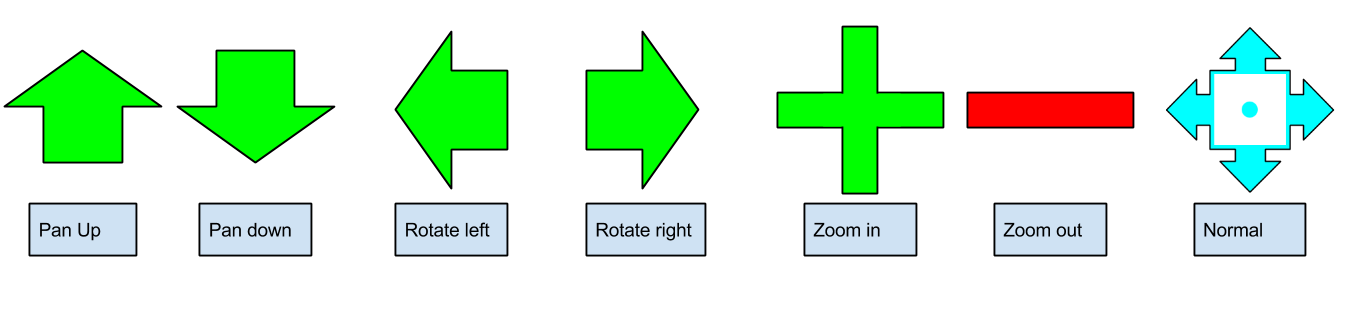
\includegraphics[width=0.9\textwidth]{images/curserImages.png}
  \caption[Example of cursor images for Kinect system]{Example of cursor images
for Kinect system to inform user of the gesture they are performing.}  
  \label{fig:cursors}
\end{figure}

No gesture design has been included for interacting with the control panel.
This is because the Microsoft Kinect sensor implementation in this visualisation
is intended as a proof of concept that interaction via gestures allows users
to access the information within the system. If the user study discussed in
Chapter \ref{C:eval}: Visualisation Evaluation shows that gesture interaction is
successful in this regard then incorporating it further could be undertaken.
 The solution designs discussed above were used for the
implementation of IKVT and are discussed in the next chapter.

\end{enumerate}